
\chapter{LeapGesture library dedicated for Leap Motion controller}\label{libraryChapter}

\section{Architecture} \label{architectureSection}

One of the main goals of creating a library for gesture recognition using Leap Motion, was simplyfying the task for developers and creating a consistent, easy to use inferface for in--applications use. A library can be treated like a black box which takes data frames as an input and responds only if a gesture from a defined set has been recognized. It was written using C++. Library is open source.

The library is divided into three main parts:
\begin{itemize}
\item process,
\item static gesture processing thread,
\item dynamic gesture processing thread.
\end{itemize}

Process part is a middle layer between user application, Leap Motion and data processing threads. It is reponsible for grabbing raw data, preprocessing it, and two--way communication with processing threads -- sending frames and receiving recognition events. That approach improves clarity of code and makes modifications easy.

After learning process has been completed, the workflow from application using the library is following:
\begin{enumerate}
  \item User creates LeapProcess and LeapListener object.
  \item User starts processing.
  \item Library starts threads for static and dynamic processing.
  \item Leap Motion reads a frame.
  \item A frame is preprocessed and sent to processing threads.
  \item If processing thread finds a gesture, an appropriate user--supplied method is invoked.
\end{enumerate}

\begin{figure}[htb]
\centering
 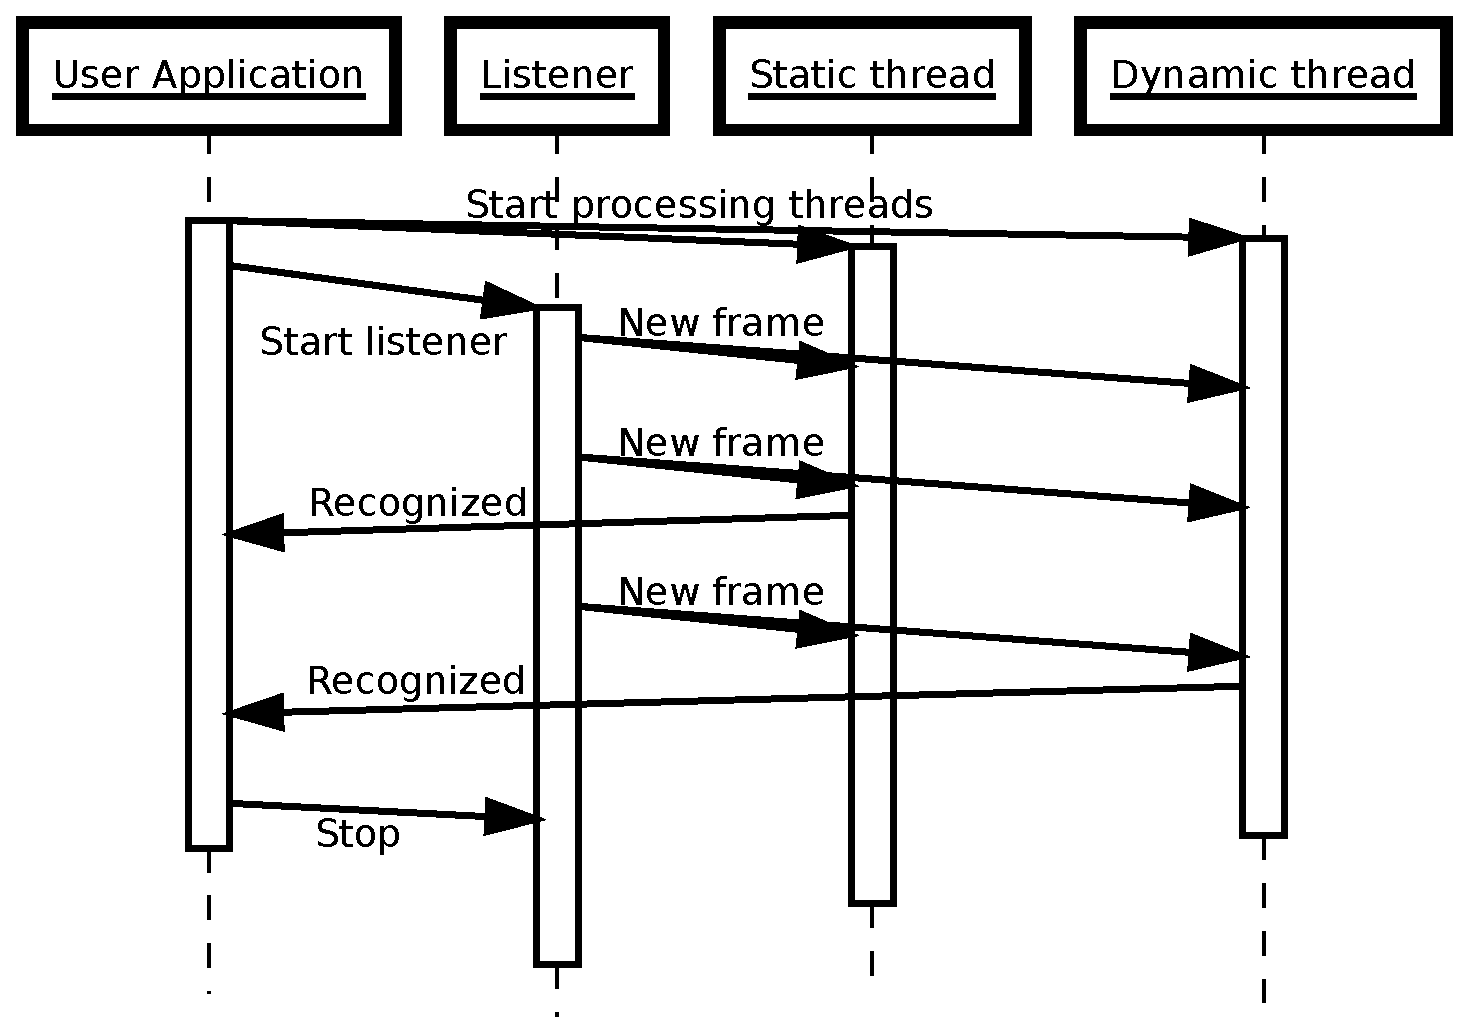
\includegraphics[width=0.8\columnwidth]{figures/timeline.eps}
 \caption[]{Sequence diagram of processing}
 \label{processingtimeline}
\end{figure}

Elements of library are following:
\begin{itemize}
\item GestureFinger, GestureHand, GestureFrame, Vertex - classes representing respectively: Frame, Hand and Finger, with additional Vertex class, which simpifies operations on 3D points
\item StorageDriver -- class supporting reading data from .lmr files
\item FileListener -- listener grabbing input data from file and feeding them to LeapProcess
\item LeapListener -- listener grabbing data from Leap Motion controller
\item LeapProcess -- class responsible for starting processing threads and two-way communication with application
\item LibLeap -- main file intented to being included by user to their project
\item LMpre -- data preprocessing
\item LMRecorder -- class responsible for translating Leap Motion API data structures to proposed by us
\item RecognizedGesture -- abstract class, user should override its methods in order to handle actions which will execute after a gesture was successfully recognized
\end{itemize}

\subsection{Model}\label{modelSubsection}

While data obtained from Leap Motion Controller are being processed, they are stored using a specially created classes representing the data. The most important class is GestureFrame, which represents a single frame captured from device. All gathered data is stored in a vector containing elements of GestureFrame type. GestureFrame holds the following information:

\begin{itemize}
\item timestamp,
\item list of data of detected hands in the frame, stored in a vector containing elements of GestureHand type.
\end{itemize}

GestureHand stores parameters of hand performing a gesture. In one instance of GestureFrame many instances of GestureHand can be stored. GestureHand holds the following information:
\begin{itemize}
\item hand id,
\item plam position,
\item stabilized palm position,
\item palm normal vector,
\item palm direction,
\item list of fingers of particular hand, stored in a vector containing elements GestureFinger type,
\item ordered value, obtained during hand sorting.
\end{itemize}

GestureFinger stores parameters of one finger. In one instance of GestureHand many instances of GestureFinger can be stored. GestureFinger contains:
\begin{itemize}
\item finger id,
\item tip position,
\item stabilized tip position,
\item finger direction,
\item finger length,
\item finger width,
\item ordered value, obtained during finger sorting.
\end{itemize}

\section{Processes}\label{processesSection}

\subsection{The learning process}
The learning process is a process of teaching LeapGesture library a new gesture by API user. First  gestures must be recorded gestures in LMR format. To obtain recordings in this format user may use Gesture Recorder --  a module included in the library, which records data from Leap Motion Controller and saves it as LMR file. When all desired gestures are prepared, the user starts the process of learning by {\color{red}[tutaj dodać informacje jak uruchomić ten prces - prawdopodobnie jakas komenda + jakies parametry typu -d uczenie gestów dynamicznych, -s uczenie gestów statycznych + pliki LMR jako argumenty]}.  

\begin{figure}[htb]
\centering
 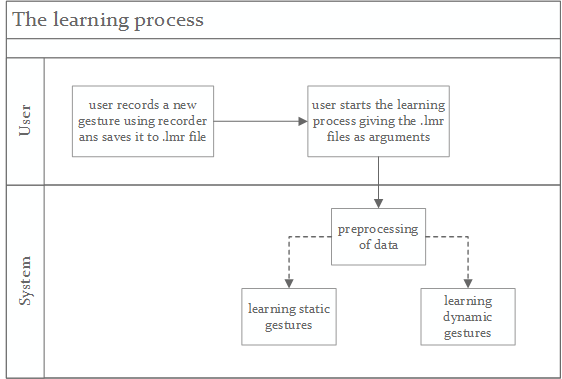
\includegraphics[width=0.75\columnwidth]{figures/learningProcess.png}
 \caption{Diagram showing the learning process for LeapGesture library}
 \label{learningprocess}
\end{figure}

The first step in the learning process, which is performed by the system is the preprocessing of data. Training data should be deprived of noise or should not have lost fingers for several frames. According to user-specified parameters, the system will learn the gesture as a static or dynamic gesture.
System uses support vector machine (SVM) for learning of static gesture. For dynamic gestures it uses Hidden Markov Model (HMM). 
The learning process for static gestures:
\begin{enumerate}
\item In the first stage, data which will be used during the learning are preprocessed.
\item Data are scaled using internal scaling module. The result of this step are scale and range files. In the scale file scaled data is stored. The range file contains information that enables to scale any data in the same way.
\item Scale file with scaled data is transmitted to a training module. Data is processed using SVM algorithm. Additionally during the learning process k-validation is performed and results are returned to the user. In the process model file is created, which is used during static gesture recognition process.
\end{enumerate}
{\color{red}[opisać learning process dla dynamicznych]}


\subsection{The recognition process}
The recognition process is a process of recognizing the gesture performed by the API user. During this process, the system uses the information obtained from the learning process. {\color{red}[Opis procesu recognition process, przedstawienie scenariusza uzycia w stosunku do architektury]}

\begin{figure}[htb]
\centering
 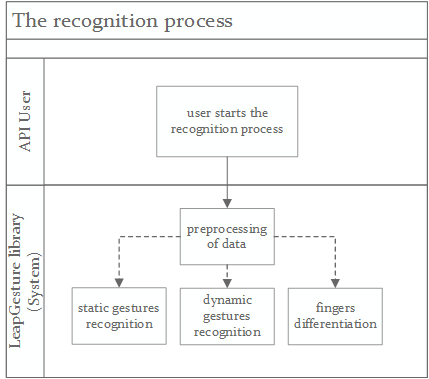
\includegraphics[width=0.6\columnwidth]{figures/recognitionProcess.png}
 \caption{Diagram showing the recognition process for LeapGesture library}
 \label{recognitionprocess}
\end{figure}

Modules handlers are implemented using the Observer pattern. For each of the modules are specified relevant events that are reported in the key moments of recognition such as: moment in which particular gesture began to be recognized, moment in which the particular gesture stopped being recognized, moment in which frame processing is finished.
The user can handle events received in specific module by implementing appropriate listener interface and adding reference to listener list in specific library module. During gesture recognition process user can use from 1 to 3 listeners. Each listener is on a separate thread.

Methods for a static gesture observer:
\begin {itemize}
\item onStart -- signals the start of the gesture,
\item onFrame -- returns a list of recognized gestures with matching probabilities,
\item onGesture -- signals the end of the gesture and returns a list of recognized gestures with matching probabilities.
\end {itemize}

Methods for a dynamic gesture observer:
\begin {itemize}
\item onStart, onFrame -- have the same purposes as in the case of static observer,
\item onGesture -- signals the end of the gesture and returns a list of recognized gestures with matching probabilities and parameter values.
\end {itemize}

Methods for a finger differentiation observer:
\begin {itemize}
\item onFrame -- returns a list of matched classes with probabilities,
\item onChange -- signals a change of fingers arrangement.
\end {itemize}

As in the learning process for recognizing static gestures system uses SVM and for dynamic gestures -- HMM. For finger differentation system uses support vector machine. However, there are other classes than those used for static gestures recogniton.

\section{Gesture recorder and visualizer}\label{recordvisualSection}
Recorder and vizualizer module is an additional part of library that allows users for easy management of gestures recordings. The recorder collects data from Leap Motion Controller, converts it into data representation described in Section~\ref and writes it to the LMR file, which is supported by the LeapGesture library. Visualizer enables users to see the recorded gestures stored in LMR format. Data gathered from Leap Motion, used to recognize gestures are very large and the data processed in the library have a specific format. Therefore, it was necessary to create an auxiliary program, that it would facilitate the work with data in the fastest and most user-friendly way.

\subsection{LMR files}
This is a file format specially developed for the LeapGesture library, supported by various modules for example by the visualizer. The file structure is as follows:
\begin{itemize}
\item Line represents one frame.
\item One frame contains: timestamp and hand parameters.
\item Hand parameters include: hand id, palm position, stabilized palm position, palm normal vector, palm direction vector and detected fingers parameters.
\item Finger parameters include: finger id, finger tip position, stabilized tip position, finger direction vector, finger length and finger width.
\end{itemize}

Example lines from LMR file:
\begin{quote}
{\color{red}4.78984}\#{\color{blue}7 -9.15495;113.759;46.292 0;0;0 -0.157914;-0.981575;0.107585 -0.0196983;-0.105799;-0.994192}f1 {\color{green} -64.0011;122.41;-28.5433 -64.831;125.304;-38.845 -0.574857;0.0254502;-0.817858 50.4269 13.0854}

{\color{red}16.6761}\#{\color{blue}7 -8.94345;113.525;46.2299 0;0;0 -0.158215;-0.981508;0.107745 -0.0193809;-0.106012;-0.994176}f1 {\color{green} -63.8514;122.144;-28.6825 -64.8135;125.248;-38.6638 -0.575861;0.0261358;-0.81713 50.4225 13.0803}

{\color{red}27.4361}\#{\color{blue}7 -8.72478;113.293;46.1443 0;0;0 -0.159539;-0.981183;0.108754 -0.0203256;-0.106877;-0.994065}f1 {\color{green} -63.5346;121.826;-28.7338 -64.7892;125.183;-38.475 -0.576776;0.0265335;-0.816472 50.3783 13.1248}
\end{quote}

This example shows a frame containing a hand with one finger exposed. The color red is used to mark frame timestamp, the blue color 
highlights information about hand, and the color green indicates information about the exposed finger.


Technical information regards LMR files:
\begin{itemize}
\item Timestamp and hands are separated by ``\#''. 
\item In specified hand occurs hand parameters and fingers. 
\item Hand parameters are separated by space, and finger are separated by ``f'' (hands parameters and fingers are separated by ``f'' too). 
\item Specified finger has parameters, which are splited by `` ''. 
\item Values in the trivalent parameters are separated by a semicolon.
\end{itemize}

\subsection{Visualizer}
Visualizer presents the contents of the LMR files. As mentioned earlier, each line of the file is a separately converted frame obtained from Leap Motion Controller. In one moment only one frame is displayed.
Almost all fields of the model are visualized:
\begin{itemize}
\item palm position,
\item palm normal vector,
\item palm direction,
\item tip position,
\item finger direction,
\item finger length.
\end{itemize}

\begin{figure}[htb]
\centering
 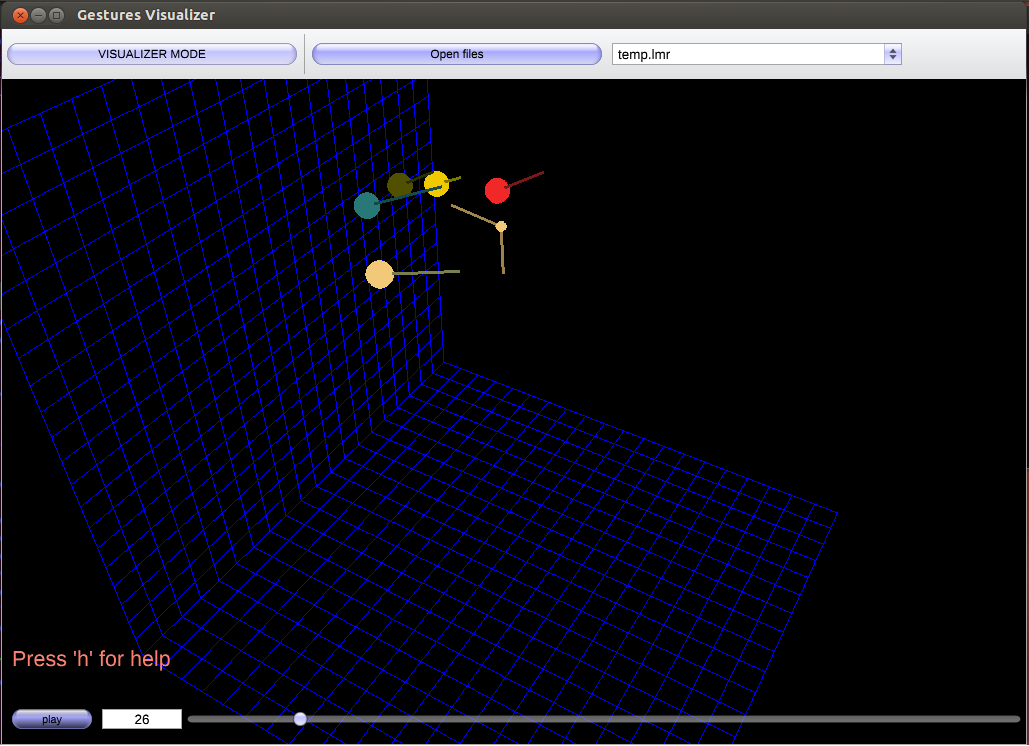
\includegraphics[width=1\columnwidth]{figures/visualizer.png}
 \caption{Screenshot of the visualizer}
 \label{visualizer}
\end{figure}

An example of parameter, which is not visualized, is finger width, in order not to obscure the image.

List of Visualizer features:
\begin{itemize}
\item Program can read the LMR files chosen by the user.
\item The user can load many files at once and select one of the recordings from the drop-down list.
\item To facilitate the user work with visualizer, program has implemented windowing interface.
\item The user has ability to rotate and zoom camera.
\item Slider is available in order to move between frames of the recording.
\item Visualizer has option to play recorded gesture, which the user can turn on and off by pressing the play/stop button.
\item There is also a button to enter the recorder mode.
\end{itemize}

\subsection{Recorder}
Recorder is part of the described module, which is responsible for collecting information from Leap Motion Controller and saving it to LMR file.

\begin{figure}[htb]
\centering
 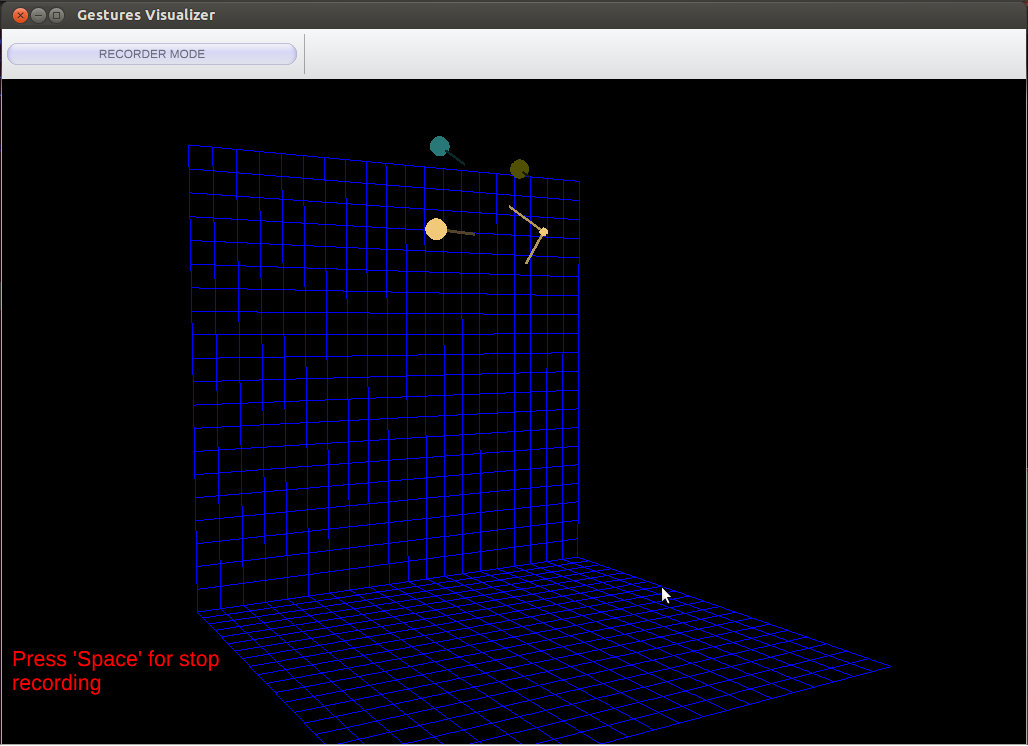
\includegraphics[width=1\columnwidth]{figures/recorder.png}
 \caption{Screenshot of the recorder}
 \label{recorder}
\end{figure}

Each frame read from the Leap Motion is captured, and then converted to the previously described model. Then the model is saved by the appropriate sub-module to LMR file. The conversion process contains also sorting hands and fingers. Hands are sorted by X coordinate of palmPosition. In the case of sorting fingers, the usual sort by the X coordinate is not enough. The order of the fingers must be independent of hand rotation, therefore a different method for fingers sorting had to be proposed. Fingers are sorted by distance between finger tip position and the plane perpendicular to the surface of the hand. The plane has to contain the direction vector of a hand. This plane can be determined using the palm position, the direction vector and a normalized normal vector of the hand.
Below is the formula for the distance ($d$) between finger tip position and designated plane.

\[ d = -(f - pp) \cdot (\hat{hd} \times \hat{hn}) \]
Where:
\begin{itemize}
    \item[] $f$: is the finger tip position
    \item[] $pp$: is the palm position
    \item[] $\hat{hd}$: is a normalized hand direction vector
    \item[] $\hat{hn}$: is a normalized hand normal vector
\end{itemize}

List of Recorder features:
\begin{itemize}
\item Turning on and off recording is done by using space key.
\item After recording window automatically appears, in which can be choosen where to save the file.
\item The recorder cooperates with the visualizer. During recording performed gesture is visualized.
\item There is a button to enter the visualizer mode.
\end{itemize}

\section{Used external libraries} \label{librariesSection}

\begin{itemize} 
\item LeapSDK -- allows to access Leap Motion device and its API
\item pthread -- library used to create lightweight processes (threads), to allow simulteanous (multithreaded) processing and provide task synchronization
\item LIBSVM -- ''A Library for Support Vector Machines'', provides SVM classifying abilities
\item Dlib -- provides linear algebra operations and machine learning ?
\item HMMlib -- a C++ library for general Hidden Markov Models
\end{itemize}

\section{Samples of code using the library dedicated for Leap Motion Controller} \label{sampleSection}

Here's an example of code required to use gesture recognition features.

\lstset{ %
language=C++,                % choose the language of the code
basicstyle=\footnotesize,       % the size of the fonts that are used for the code
numbers=left,                   % where to put the line-numbers
numberstyle=\footnotesize,      % the size of the fonts that are used for the line-numbers
stepnumber=1,                   % the step between two line-numbers. If it is 1 each line will be numbered
numbersep=5pt,                  % how far the line-numbers are from the code
backgroundcolor=\color{white},  % choose the background color. You must add \usepackage{color}
showspaces=false,               % show spaces adding particular underscores
showstringspaces=false,         % underline spaces within strings
showtabs=false,                 % show tabs within strings adding particular underscores
frame=single,           % adds a frame around the code
tabsize=2,          % sets default tabsize to 2 spaces
captionpos=b,           % sets the caption-position to bottom
breaklines=true,        % sets automatic line breaking
breakatwhitespace=false,    % sets if automatic breaks should only happen at whitespace
escapeinside={\%*}{*)}          % if you want to add a comment within your code
}
\begin{lstlisting}
// specifies method which will be executed after successful recognition
class MyGestures: public RecognizedGestureListener {

	void onStaticRecognized() {
		cout << "Recognized static gesture!" << endl;
	}

	void onDynamicRecognized() {
		cout << "Recognized dynamic gesture!" << endl;
	}

};

int main(int argc, char **argv) {

	// create instance of recognized gesture actions
	MyGestures *gst = new MyGestures();

	// create new data processor (for static gestures only)
	LeapProcess *process = new LeapProcess(gst, true, false);

	// specify settings: path where model with given name is located
	StaticSettings settings("/home/oli", "testmodel");
	process->staticSettings = settings;
	
	// create a listener and attach it to a process
	LeapListener listener(3);	// 3 = radius of preprocessing windows
	listener.attachToProcess(process);
	
	// create a Leap Motion controller object and direct its data output to a listener
	Controller c(listener);

	// start processing
	process->start();
	
	// as processing works in a separate thread, application can now perform other tasks
	cin.get();
	
	// stop processing
	c.removeListener(listener);

}
\end{lstlisting}
